\teaser{
	\centering
	\vspace{-1cm}
	\addtolength{\tabcolsep}{-4.5pt}
	\newlength{\insetLen}
	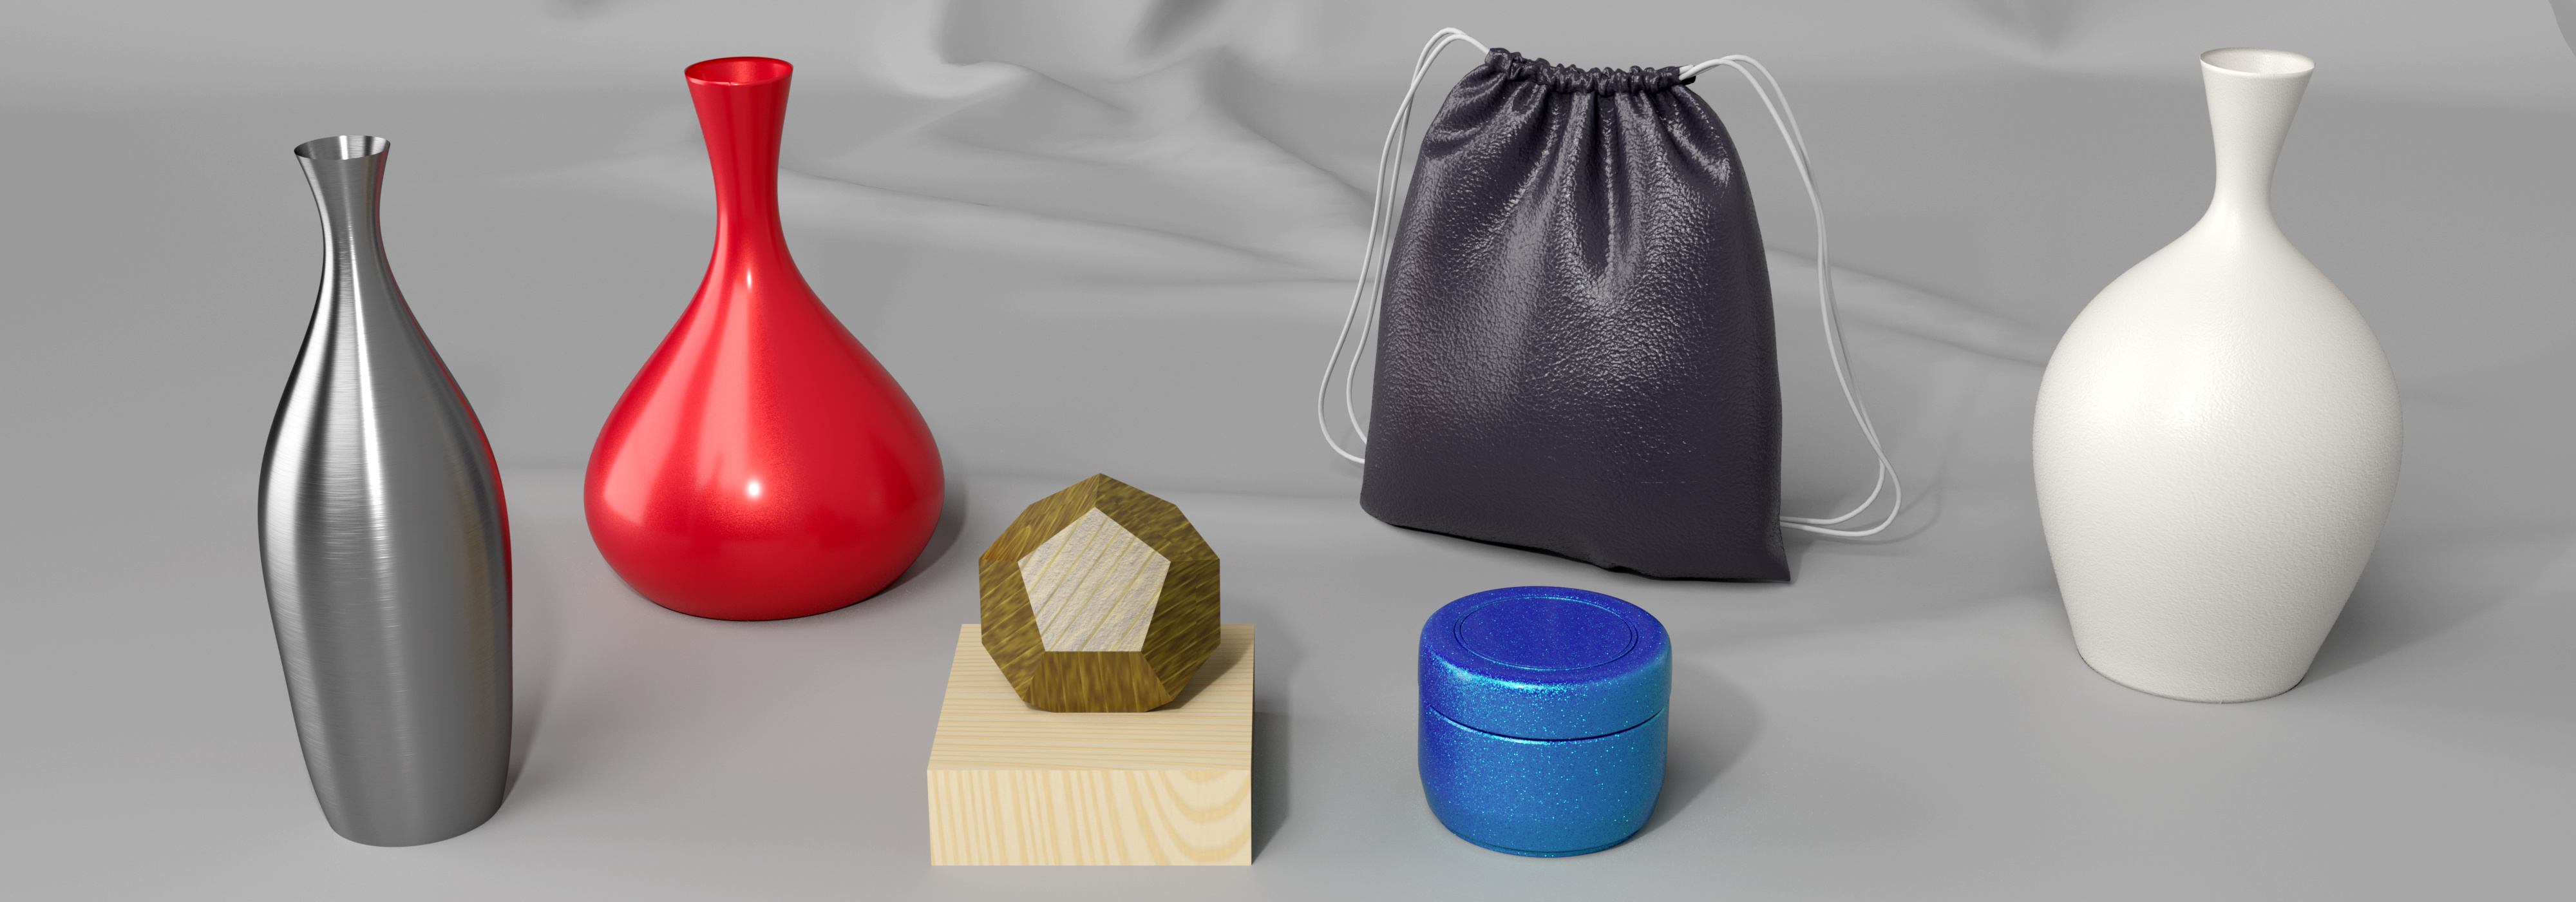
\includegraphics[width=0.98\textwidth]{fig1-2/teaser.jpg}\\[2pt]
	\setlength{\insetLen}{0.132\textwidth}
	\begin{tabular}{cccccccc}
		\raisebox{7pt}{\rotatebox{90}{\small \bfseries Input}} &
		\adjincludegraphics[width=\insetLen,trim={0 {.2\height} 0 {.2\height}},clip]{fig7/5_metal_3/target.jpg} &
		\adjincludegraphics[width=\insetLen,trim={0 {.2\height} 0 {.2\height}},clip]{fig7/4_flake_4/target.jpg} &
		\adjincludegraphics[width=\insetLen,trim={0 {.2\height} 0 {.2\height}},clip]{fig7/6_wood_4/target.jpg} &
		\adjincludegraphics[width=\insetLen,trim={0 {.2\height} 0 {.2\height}},clip]{fig7/6_wood_5/target.jpg} &
		\adjincludegraphics[width=\insetLen,trim={0 {.2\height} 0 {.2\height}},clip]{fig5/4_flake_1/target.jpg} &
		\adjincludegraphics[width=\insetLen,trim={0 {.2\height} 0 {.2\height}},clip]{fig7/2_leather_3/target.jpg} &
		\adjincludegraphics[width=\insetLen,trim={0 {.2\height} 0 {.2\height}},clip]{fig7/1_bump_4/target.jpg}
		\\
		\raisebox{3pt}{\rotatebox{90}{\small \bfseries Rendered}} &
		\adjincludegraphics[width=\insetLen,trim={0 {.2\height} 0 {.2\height}},clip]{fig7/5_metal_3/good1.jpg} &
		\adjincludegraphics[width=\insetLen,trim={0 {.2\height} 0 {.2\height}},clip]{fig7/4_flake_4/good1.jpg} &
		\adjincludegraphics[width=\insetLen,trim={0 {.2\height} 0 {.2\height}},clip]{fig7/6_wood_4/good1.jpg} &
		\adjincludegraphics[width=\insetLen,trim={0 {.2\height} 0 {.2\height}},clip]{fig7/6_wood_5/good1.jpg} &
		\adjincludegraphics[width=\insetLen,trim={0 {.2\height} 0 {.2\height}},clip]{fig5/4_flake_1/good1.jpg} &
		\adjincludegraphics[width=\insetLen,trim={0 {.2\height} 0 {.2\height}},clip]{fig7/2_leather_3/good1.jpg} &
		\adjincludegraphics[width=\insetLen,trim={0 {.2\height} 0 {.2\height}},clip]{fig7/1_bump_4/good1.jpg}
	\end{tabular}
	\captionsetup{labelfont=bf,textfont=it}
	\caption{
			A scene rendered with material parameters estimated using our method: bumpy dielectrics, leather, plaster, wood, brushed metal, and metallic paint. The insets show a few examples of the input (target) images, and renderings produced using our procedural models with parameters found by Bayesian posterior sampling.
		\vspace{3mm}
 	}
	\label{fig:teaser}
}
